\section{Desarrollo}
% Metodologia / Desarrollo

Para nuestro desarollo partimos de las consideraciones iniciales como los paquetes a empacar, la capacidad de los contenedores y los parámetros del 
algoritmo de colonia de hormigas.

\subsection{Consideraciones iniciales}

Primeramente se define la instancia del problema y los parámetros generales del algoritmo. Se especifican:

\begin{itemize}
    \item El conjunto de objetos a empacar:Para lo cual generamos un arreglo de 1000 paquetes con tamaños aleatorios entre los 5 tipos definidos,
    donde cada dato corresponde al tamaño de un paquete como se menciona en la sección~\ref{Problema}.
    \item La capacidad de los contenedores, $C = 12$, ya que el trailer tiene 2.4 m de ancho y cada 
    paquete ocupa 0.8 m, lo que permite formar 3 columnas. Cada columna tiene 12 m de largo, por lo que 
    su capacidad es de 12 unidades.
    \item Se calcula la suma total del tamaño de los 1000 paquetes.  
    \item Se obtiene el número mínimo de columnas necesarias dividiendo esta suma entre la 
    capacidad de una columna ($C = 12$) y aplicando redondeo hacia arriba:
    \[
        \text{min\_columnas} = \left\lceil \frac{\sum p_i}{C} \right\rceil.
    \]
    \item Para evitar que el algoritmo se quede sin opciones y permitir mayor exploración, se 
    introduce un factor de holgura de 1.2, es decir, se usa un 20\% más de columnas que el 
    mínimo teórico:
    \[
        \text{n\_columnas} = \left\lceil 1.2 \times \text{min\_columnas} \right\rceil.
    \]
    \item Como cada contenedor físico está compuesto por 3 columnas (debido al ancho disponible 
    del tráiler), se ajusta el número total para que siempre sea múltiplo de 3.
    \item Finalmente, cada grupo de tres columnas se etiqueta como un contenedor con columnas 
    internas, por ejemplo: \texttt{Cont\_3\_Col\_1}, \texttt{Cont\_3\_Col\_2}, \texttt{Cont\_3\_Col\_3}.
    \item Los parámetros del algoritmo de colonia de hormigas:
    \[
    \alpha = 1.0, \quad
    \beta = 2.0, \quad
    \rho = 0.5, \quad
    Q = 1.0,
    \]
\end{itemize}

\subsection{Codificación}

Cada solución se representa como un vector donde la posición indica el objeto y el valor indica el contenedor asignado. Por ejemplo:

\[
\mathbf{s} = [A, A, B, C, B, D, C]
\]

indica que el primer y segundo objeto van al contenedor A, el tercero y quinto al B, el cuarto y séptimo al C, etc. Es decir esta representación se 
maneja como una lista o arreglo de enteros (índices de contenedor).

Con lo cual debemos calcular para cada contenedor:

\begin{itemize}
    \item La suma de tamaños de los objetos asignados (carga).
    \item Evitando que se viole la capacidad máxima $C$.
\end{itemize}

\subsection{Inicialización de feromonas y heurística}

Se inicializa una matriz de feromonas $\tau_{ij}$ de tamaño 
\[
\text{(número de objetos)} \times \text{(número de contenedores)},
\]
es decir,
\[
\text{(7)} \times \text{(5)},
\]
donde cada entrada $\tau_{ij}$ representa la cantidad de feromona asociada a asignar el objeto $i$ al contenedor $j$. Inicialmente se suele utilizar un valor constante:

\[
\tau_{ij} = \tau_0, \quad \forall i,j,
\]

para no sesgar la búsqueda hacia ningún contenedor específico.

La heurística $\eta_{ij}$ se define en función del espacio restante en el contenedor $j$ si se colocara el objeto $i$. Como se menciona en 
la ecuacion~\ref{eq: heuristica}

Esto favorece asignaciones que llenan mejor el contenedor sin exceder la capacidad. Esta heurística se recalcula dinámicamente mientras la hormiga construye su solución, ya que el espacio disponible cambia conforme se asignan objetos.

\begin{figure}[H]
    \centering
    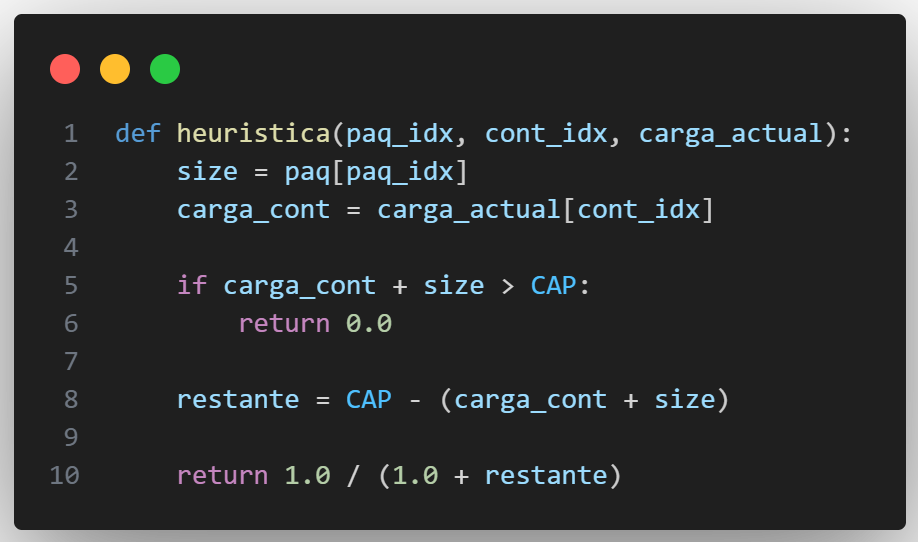
\includegraphics[width=0.6\textwidth]{rsc/img/des/heuristica.png}
    \caption{Funcion heuristica utilizada en python}\label{fig:funcion_heuristica}
\end{figure}

\subsection{Construcción de soluciones por las hormigas}

En cada iteración, cada hormiga construye una solución asignando los objetos uno a uno. Para cada objeto $i$, la hormiga evalúa los 
contenedores factibles (aquellos donde el objeto cabe sin exceder la capacidad) y selecciona un contenedor $j$ de acuerdo con la probabilidad:

\begin{equation}
P_{ij} = 
\frac{\tau_{ij}^{\alpha} \, \eta_{ij}^{\beta}}
{\sum\limits_{l \in \text{Contenedores válidos}} \tau_{il}^{\alpha} \, \eta_{il}^{\beta}}.
\end{equation}

Esta regla combina la información histórica (feromonas) con la información local (heurística).
\begin{figure}[H]
    \centering
    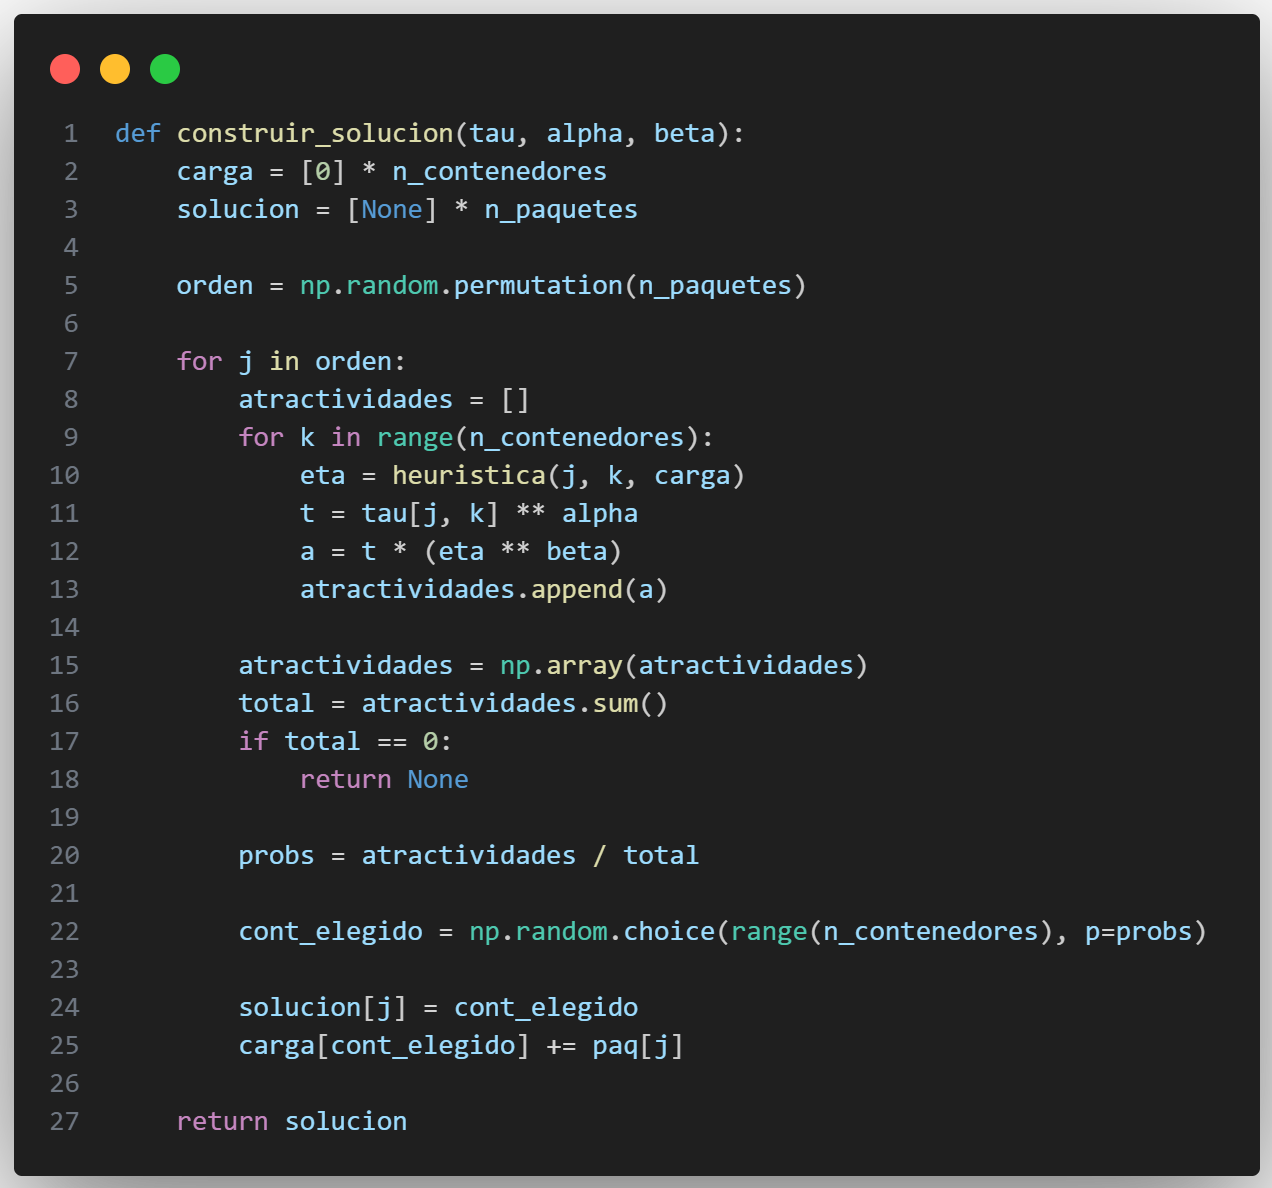
\includegraphics[width=0.6\textwidth]{rsc/img/des/const_sol.png}
    \caption{Funcion Construcción de Solución utilizada en python}\label{fig:funcion_cost_sol}
\end{figure}


\subsection{Evaluación de la función de aptitud}

Una vez que una hormiga ha construido su solución completa, se evalúa mediante una función de aptitud diseñada para:

\begin{itemize}
    \item Maximizar el uso de capacidad de los contenedores empleados.
    \item Minimizar el número de contenedores utilizados.
\end{itemize}

Se emplea una función de la forma:

\begin{equation}
f = \frac{2}{N} \sum_{i=1}^{N} \frac{F_i}{C},
\end{equation}

donde $N$ es el número de contenedores usados, $F_i$ es la suma de tamaños de los objetos en el contenedor $i$ y $C$ es la capacidad de cada contenedor. Esta función está normalizada de manera que valores cercanos a 1 indican soluciones donde los contenedores están muy bien llenos (con poco espacio desperdiciado).

Además, se pueden añadir penalizaciones si algún contenedor excede su capacidad o si se supera un número máximo de contenedores.

\begin{figure}[H]
    \centering
    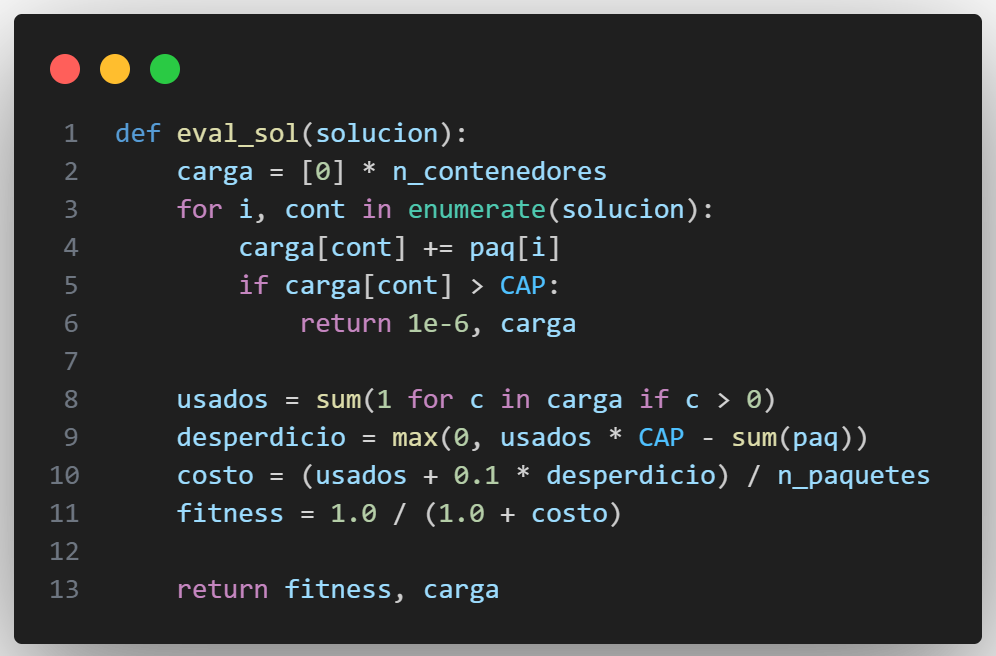
\includegraphics[width=0.6\textwidth]{rsc/img/des/eval_sol.png}
    \caption{Funcion Evaluación de Solución utilizada en python}\label{fig:funcion_eval_sol}
\end{figure}

\subsection{Actualización de feromonas}

Al finalizar la construcción y evaluación de todas las soluciones en una iteración, se actualiza la matriz de feromonas en dos etapas:

\begin{enumerate}
    \item \textbf{Evaporación global:}
    \begin{equation}
        \tau_{ij} \leftarrow (1 - \rho)\,\tau_{ij},
    \end{equation}
    con $\rho = 0.5$ como tasa de evaporación. Esto evita que las rutas antiguas dominen la búsqueda.
    \item \textbf{Depósito de feromonas:} se refuerzan las asignaciones objeto–contenedor pertenecientes a la mejor solución (ya sea la mejor de la iteración o la mejor global):
    \begin{equation}
    \tau_{ij} \leftarrow \tau_{ij} + \Delta \tau_{ij},
    \end{equation}
    donde
    \begin{equation}
    \Delta \tau_{ij} = 
    \begin{cases}
        \displaystyle \frac{Q}{f_{\text{best}}}, & \text{si la asignación $(i,j)$ está en la mejor solución},\\[4pt]
        0, & \text{en otro caso},
    \end{cases}
    \end{equation}
    y $Q = 1.0$ es la cantidad base de feromona depositada, mientras que $f_{\text{best}}$ es la aptitud de la mejor solución.
\end{enumerate}

La lógica de actualización se implementa en una función auxiliar que recibe la solución ganadora y la matriz de feromonas, aplicando evaporación y depósito de forma vectorizada cuando es posible.

\subsection{Ejecución del algoritmo y recolección de métricas}

Por ultimo corremos nuestro algoritmo de colonia de hormigas asi como una funcion auxiliar para recolectar las metricas en cada iteración.

\begin{figure}[H]
    \centering
    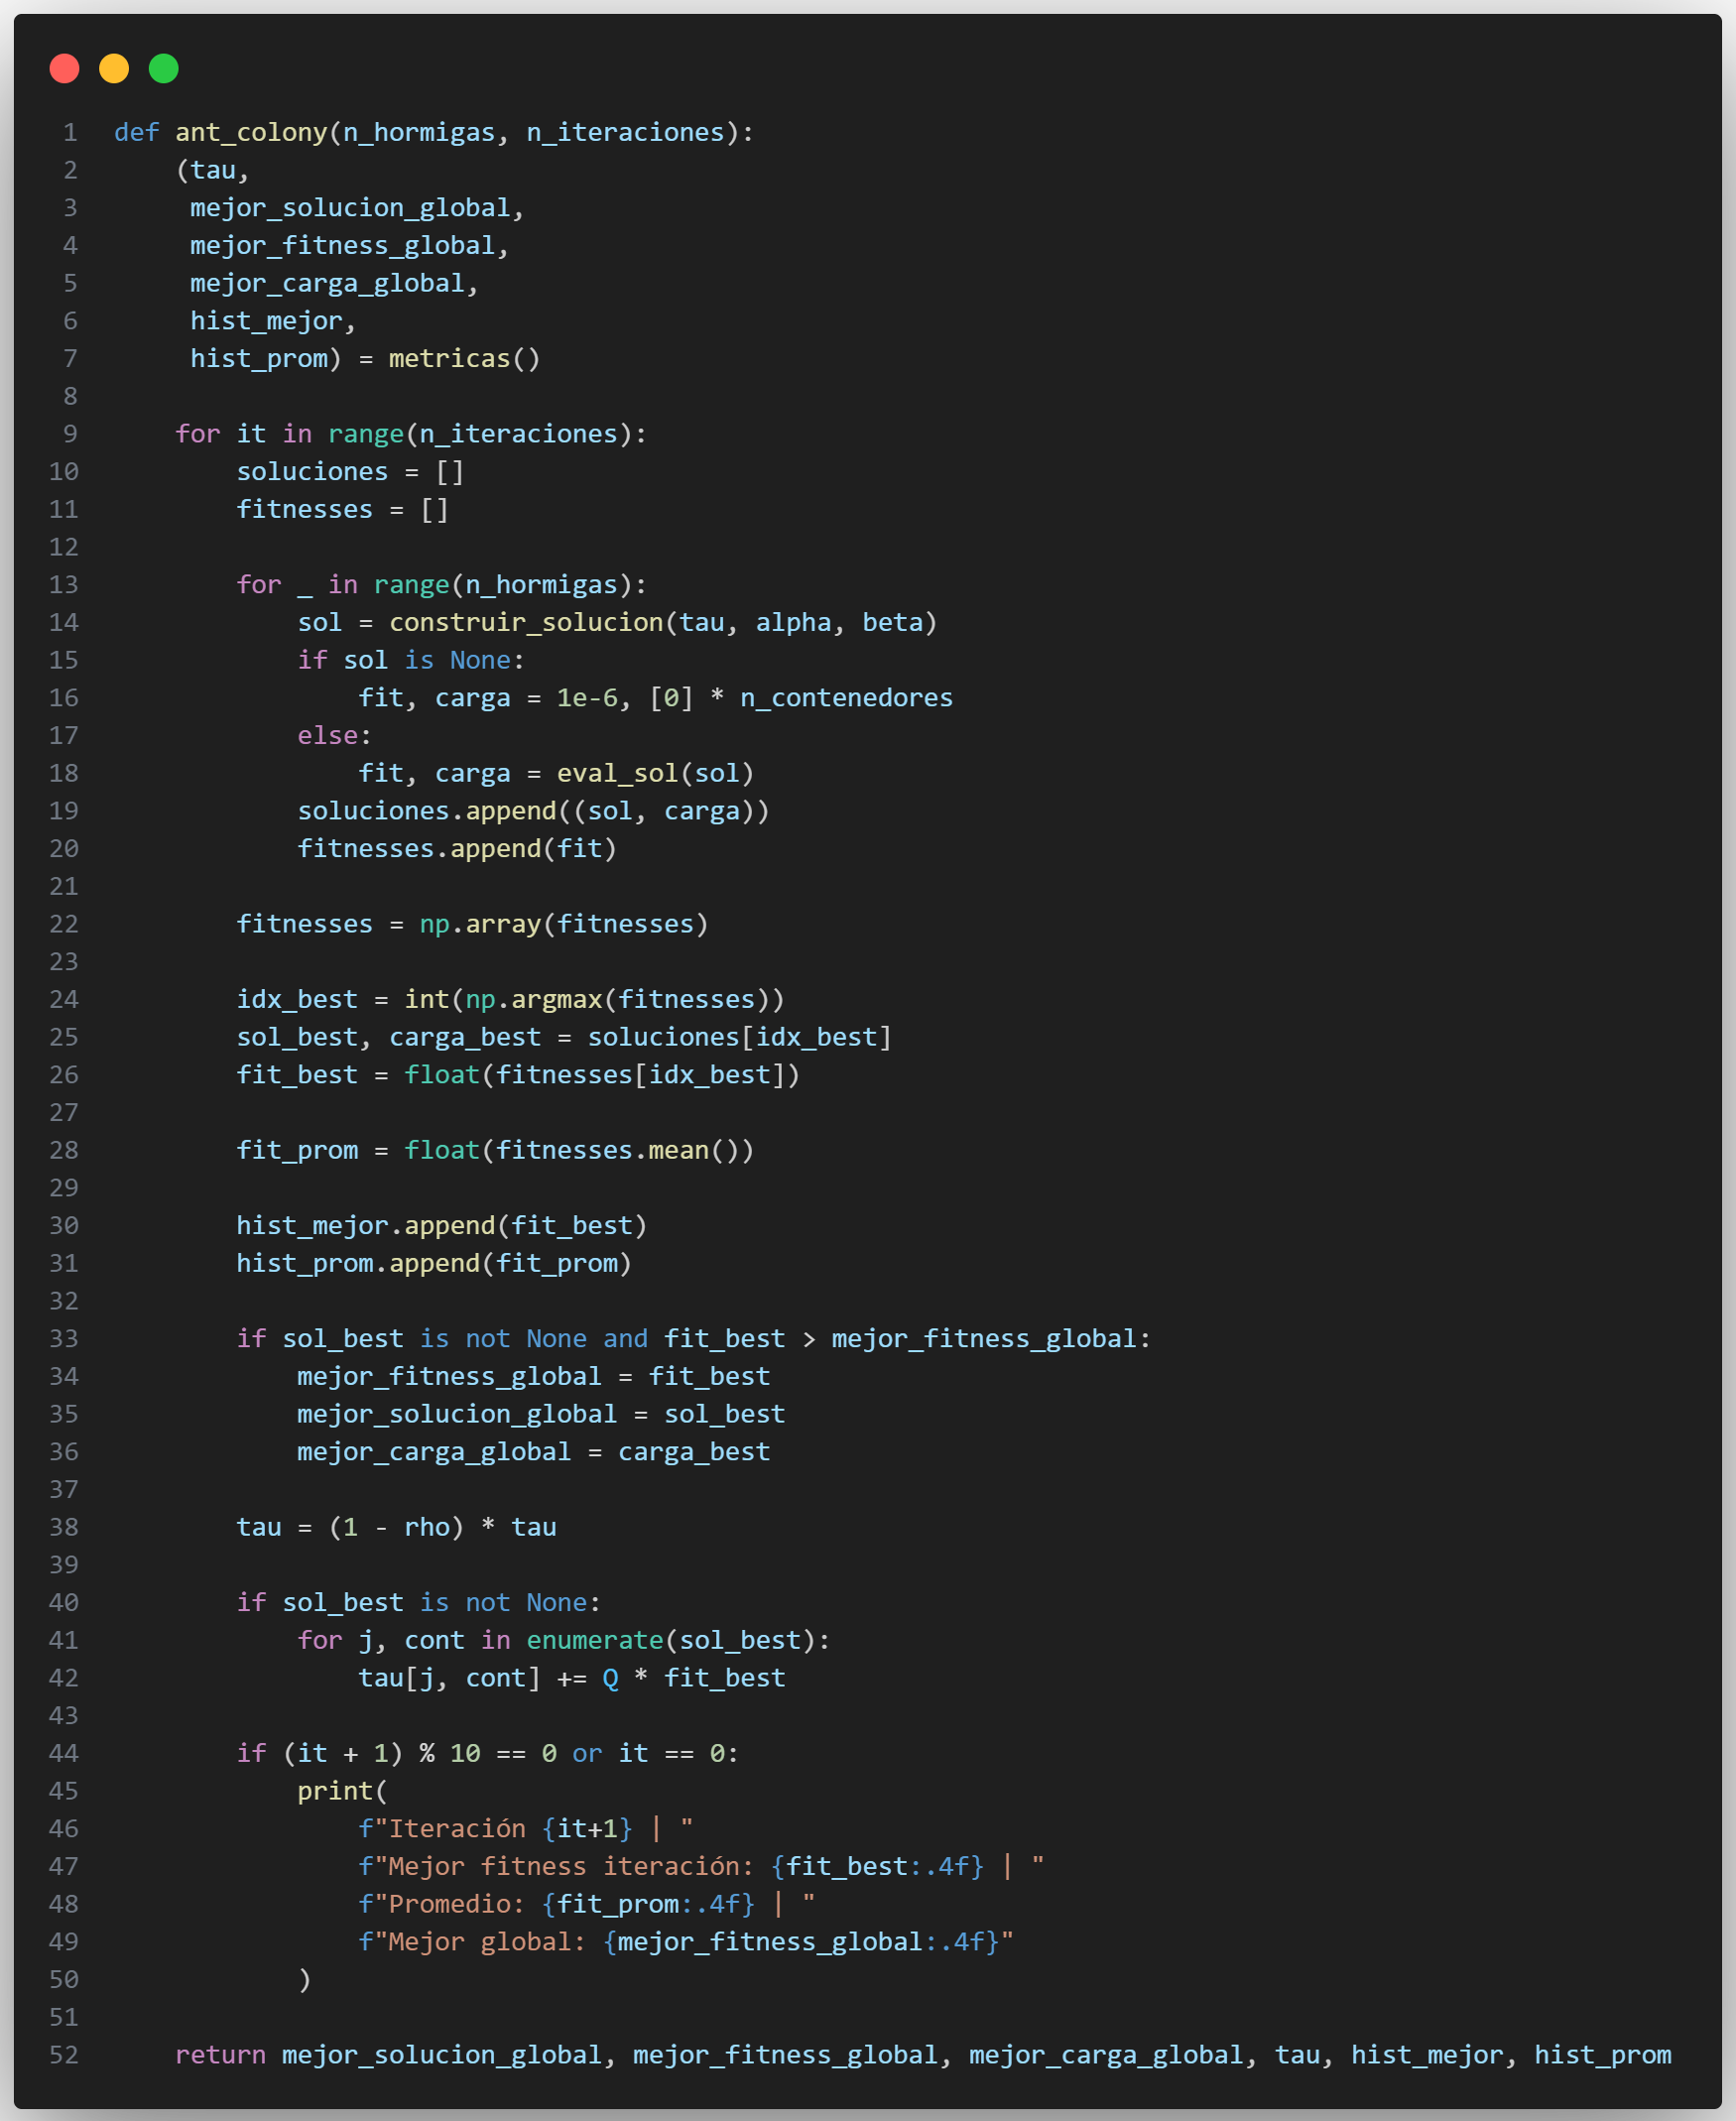
\includegraphics[width=0.6\textwidth]{rsc/img/des/ant_colony.png}
    \caption{Funcion Ant Colony utilizada en python}\label{fig:funcion_ant_colony}
\end{figure}

\begin{figure}[H]
    \centering
    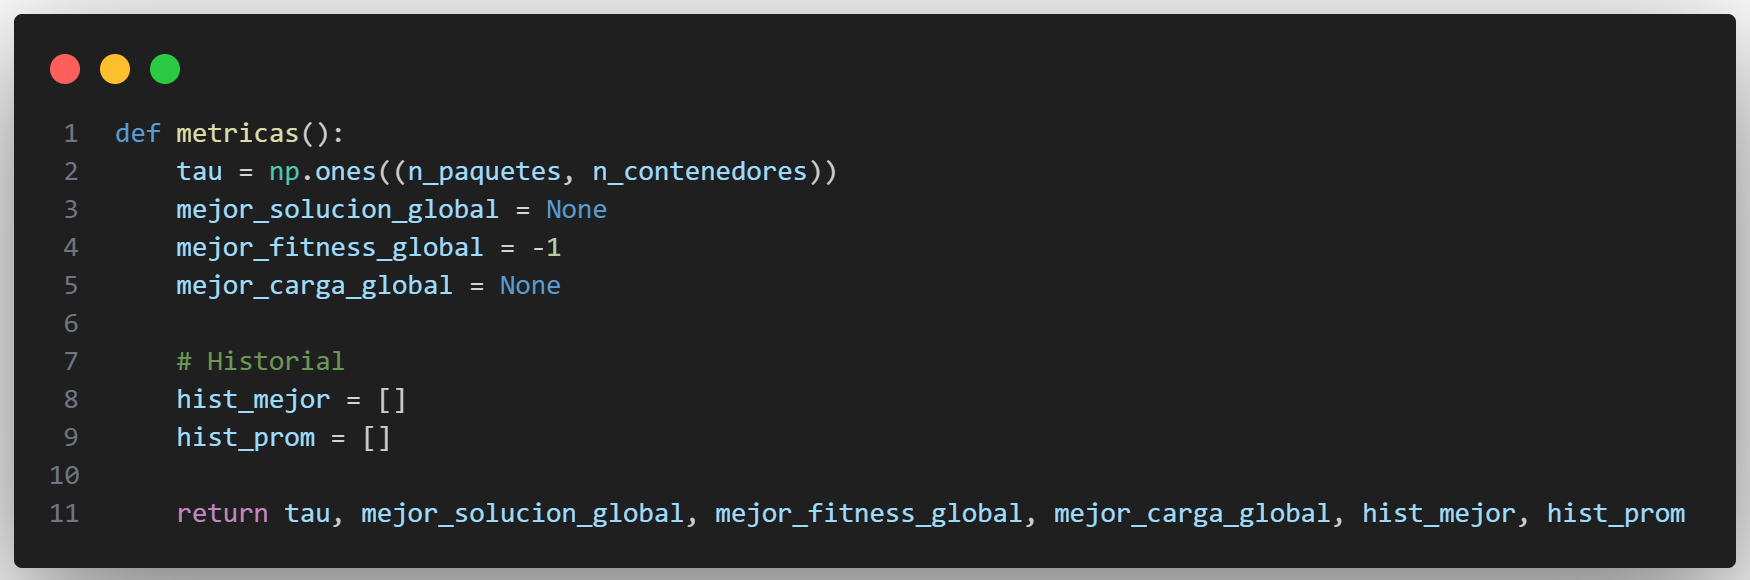
\includegraphics[width=0.6\textwidth]{rsc/img/des/metricas.png}
    \caption{Funcion Metricas utilizada en python}\label{fig:funcion_metricas}
\end{figure}

En cada iteración se ejecutan los siguientes pasos:

\begin{enumerate}
    \item Inicializar una lista vacía de soluciones y aptitudes.
    \item Para cada hormiga:
    \begin{enumerate}
        \item Construir una solución completa (Figura~\ref{fig:funcion_cost_sol}).
        \item Evaluar su aptitud (Figura~\ref{fig:funcion_eval_sol}).
    \end{enumerate}
    \item Actualizar la mejor solución global si alguna hormiga la mejora.
    \item Actualizar las feromonas.
    \item Llamar a la función metricas (Figura~\ref{fig:funcion_metricas}) para registrar:
    \begin{itemize}
        \item La mejor aptitud de la iteración.
        \item El promedio de aptitud de todas las hormigas.
        \item Información adicional sobre la carga de los contenedores.
    \end{itemize}
\end{enumerate}
